\subsection{LeNet-5}
\begin{frame}{}
    \LARGE CNN Architectures: \textbf{LeNet-5}
\end{frame}

% LeNet-5
\begin{frame}{LeNet-5}
    \begin{figure}
        \centering
        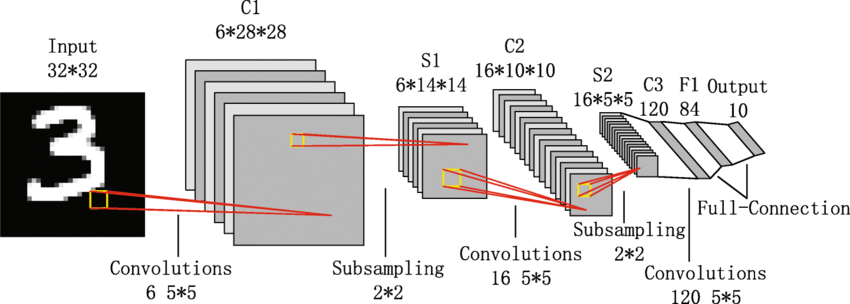
\includegraphics[width=0.8\textwidth,height=0.4\textheight,keepaspectratio]{images/cnn/lenet5.png}
        \caption*{LeNet-5 architecture.}
    \end{figure}
    {\small
        \begin{itemize}
            \item LeNet-5 is a pioneering convolutional neural network (CNN) architecture developed by Yann LeCun and his collaborators in the late 1980s and early 1990s.
            \item It was built to recognize handwritten digits, like those in the MNIST dataset.
            \item The network uses layers that look for patterns (convolution), shrink images (pooling), and finally make decisions (fully connected layers).
            \item LeNet-5 introduced ideas like using filters to find features and pooling to reduce size, which are now common in modern CNNs.
        \end{itemize}
    }
\end{frame}